\chapter{机器学习算法一致收敛基础理论}
\label{chap:edbed}
\section{引言}
本章给出机器学习算法一致收敛基础理论, 这些理论对于后续章节中阐述具体算法起到至关重要的指导作用。因为后续章节的工作都建立在机器学习算法的输出结果之上而展开的研究, 所以对于具体机器学习算法并不会展开详细的介绍, 仅仅从理论层面对底层机器学习算法给出分析。

关于机器学习算法的理论阐述, 最后归约为基于经验数据的相依关系估计问题\citep{vapnik1982}。这一问题由Vapnik和Chervonenkis完整给出\citep{vapnik1974,vapnik1979,Vapnik2006,Chervonenkis2013}。Vapnik公理化定义“模式”, 给出“识别”的定义并且提出采用“广义肖像法”实现模式识别问题的解答\citep{vapnik1962,vapnik1963,vapnik1964On,vapnik1964}。对于泛函依赖关系估计问题, 按照泛函分析理论都抽象为相同的模型来考虑, 即在所有可能的依赖关系中需要找到某函数关系, 此函数关系是满足给定量化评价标准下的最佳函数关系。形式化而言, 即对于向量空间 $Z$, 诸函数的集合 $\{g(z), z \in Z\}$所有可能的依赖关系的类是给定的。定义某泛函表达式
\begin{align}\label{1.1}
I = I(g)
\end{align}
作为选择依赖关系的量化指标。那么需要在集合 $\{g(z)\}$ 中搜索使得泛函 (\ref{1.1}) 最小化的函数 $g^{*}(z)$。在这种情形下,当给出函数集合$\{g(z)\}$和泛函$I(g)$的确切数学表达式时, 寻找使泛函$I(g)$最小化的函数$g^{*}(z)$的问题就转化为变分法的求解问题\citep{Hilbert1950,mmp-1953,mmp-1962,Marx1881}。

然而就学习问题而言, 统计学习理论将之归约为根据经验数据的相依关系估计问题\citep{vapnik1974,Faffelberger1980}。即在所有可能的泛函依赖关系中选择一个在满足给定的量化评价标准下最优函数(诸函数是由机器实施的)。形式化而言, 即当概率密度函数$P(z)$定义在向量空间$Z$, 泛函关系定义为下列数学期望
\begin{align}\label{1.2}
I(g) = \int \Phi(z,g(z))P(z)dz.
\end{align}
那么所考虑的问题就是当概率密度函数 $P(z)$未知, 但已知观测样本
\begin{align}\label{1.3}
z_1,\ldots,z_l
\end{align}
来源于服从密度函数$P(z)$的随机独立试验时,最小化泛函 (\ref{1.2})的问题。

对于最小化期望风险泛函问题, 诸函数的类 $\{g(z)\}$是以参数形式$\{g(z,\alpha)\}$给出的, 其中这里参数$\alpha$是属于集合$\Lambda$的。对于具体的参数取值$\alpha = \alpha^{*}$, 其定义属于函数类$g(z,\alpha)$的某具体函数$g(z, \alpha^{*})$。就学习问题而言, 搜索所需函数等同于确立所求参数$\alpha$的值。特别需要指出的是, 问题的研究并不局限在仅由某几个参数确定的函数类, 而是集合 $\Lambda$ 的参数 $\alpha$ 可以是任意的, 比如可以是诸标量的集合,或者诸向量的集合,也可以是任意抽象元素的集合。例如在神经网络中,这里的集合 $\Lambda$就是网络节点的集合。

现在可以将泛函(\ref{1.2})重新用新的术语写出, 即
\begin{align}\label{1.4}
I(\alpha) = \int Q(z,\alpha)P(z)dz, \alpha \in \Lambda,
\end{align}
其中,
\begin{align}
Q(z,\alpha) = \Phi(z,g(z,\alpha)).
\end{align}
这里的函数 $Q(z,\alpha)$称为损失函数。

现在考虑具体的情况, 即向量空间 $z$ 有$n+1$ 个坐标, 其中分别是标量 $y$ 以及 $n$ 个坐标的数据向量 $x$。损失函数 $Q(z,\alpha)$ 按下列表达式给出
\begin{align}
Q(z,\alpha) = \Phi(y - F(x,\alpha)),
\end{align}
其中,这里函数 $F(x,\alpha)$ 是参数化的诸函数的类。现在的问题是最小化下列泛函
\begin{align}\label{1.5}
I(\alpha) = \int \Phi(y-f(x,\alpha))P(x,y)dxdy
\end{align}
而所面对情形是这里的概率密度 $P(x,y)$ 未知, 但随机独立的训练序列样本给定
\begin{align}\label{1.6}
x_1,y_1; \ldots; x_l,y_l.
\end{align}

将基于经验数据(\ref{1.6})来最小化泛函(\ref{1.5})的问题称为基于经验数据的相依关系估计, 亦称作统计学习问题。


统计学习问题的理论阐述是20世纪50年代末期提出\citep{Rosenblatt1962,Novikoff1962,vapnik1963,vapnik1964,vapnik1964On,vapnik1968,vapnik1971,vapnik1974,vapnik1979}, 这一类问题的数学形式化可以表述为:按照图 \ref{fig:power-right}所示, 这里有三个要素:
\begin{enumerate}
\item 数据的生成器 $G$,
\item 目标算子或监督器 $S$,
\item 学习机器 $LM$。
\end{enumerate}

统计学习理论中关于机器学习算法的学习问题设定属于现象学学习模型\citep{Vapnik-rethinking-2018,wangdefeng2005}, 即在由概率密度函数 $P(x)$ 所刻画的环境条件下, 数据 $x$ 随机且独立地出现, 学习机制是把数据划分为 $k$ 个不同的类别。假设学习机器按照条件概率分布函数 $P(y | x), y = \{0,1\}$, ($y=0$ 表示将 $x$ 划分为第一类,  $y=1$ 表示划分为第二类)进行分类。给定参数化泛函集合 $F(x,\alpha)$和观测到的$l$对数据
\begin{align}
x_1, y_1; \ldots; x_l, y_l,
\end{align}
其中, 这里的$x$表示学习环境, $y$为学习反馈。学习过程就是在集合$F(x,\alpha)$中选择一个函数使得其分类错误的概率是集合中其他分类器中最小的。也就是说, 必须取得下列泛函的最小值
\begin{align}
I(\alpha) = \int_{X,y}^{} (y - F(x,\alpha))^2P(x,y)dxdy.
\end{align}
其中,这里的函数$P(x,y) = P(y | x)P(x)$ 是定义在空间$X, y$上的关于数据对$x, y$的联合概率密度函数。这样一来学习问题被归约为基于经验数据的最小化期望风险问题。

\begin{figure}
\centering
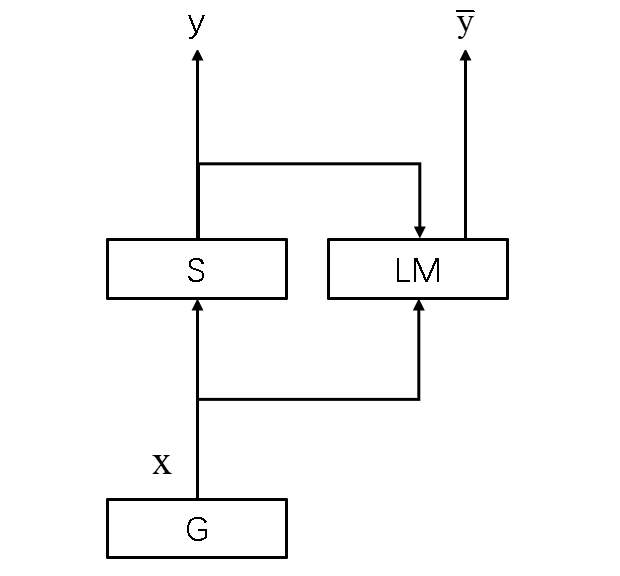
\includegraphics[width=.4\linewidth]{Img/chapter1/power-right.png}
\caption{现象学学习理论模型示意图}
\label{fig:power-right}
\end{figure}

\section{将学习问题归约为最小化经验风险泛函问题}
统计学在处理这一问题时,将此问题与估计诸概率密度函数问题相关联。按照统计学处理思路, 下列期望风险泛函
\begin{align}\label{ch6.1}
I(\alpha)=\int(y-F(x, \alpha))^{2} P(x, y) d x ~d y
\end{align}
在基于下列经验数据
\begin{align}\label{ch6.2}
x_{1}, y_{1} ; \ldots ; x_{l}, y_{l}
\end{align}
最小化的问题被归约为基于样本数据(\ref{ch6.2})估计密度函数$\hat{P}(x,y)$, 然后再求解关下列泛函的最小化问题
\begin{align}
I_{\mathrm{emp}}(\alpha)=\int(y-F(x, \alpha))^{2} \hat{P}(x, y) d x ~d y.
\end{align}

\citet{vapnik1982}已经完整阐明, 用这种方法最小化风险泛函(\ref{ch6.1})通常是不合理的。因为相较于最小化期望风险(\ref{ch6.1}), 密度函数的估计问题通常是更艰难的问题。只有当拥有关于这一密度函数$P(x,y)$足够多的、可用的先验信息时, 函数$P(x,y)$的参数方才有可能确定, 此时传统统计学的方法才能够勉强的、似是而非的执行\citep{Vapnik2006}。然而对于特定的现实问题其密度函数$P(x,y)$是未知的, 因此统计学处理这一问题就始终扭结在如何提供一个很好的密度函数的假设上。

统计学习理论处理这类问题则无需任何分布假设。统计学习理论的基本原则是对于最小化期望风险泛函问题, 当期望风险泛函(\ref{ch6.1})取得最小值的时候, 由随机独立样本(\ref{ch6.2})构建的下列经验风险泛函
\begin{align}\label{ch6.3}
I_{\mathrm{emp}}(\alpha)=\frac{1}{l} \sum_{i=1}^{l}\left(y_{i}-F\left(x_{i}, \alpha\right)\right)^{2},
\end{align}
也取得最小值。令经验风险泛函(\ref{ch6.3})取得的最小值为 $F(x,\alpha_{emp})$。那么关键的问题就是要阐明, 到底在什么时候, 经验风险泛函的最小值$F(x,\alpha_{emp})$能逼近期望风险泛函的最小值$F(x,\alpha_0)$, 而后者正好就是在函数族$F(x,\alpha)$中能够最小化表达式(\ref{ch6.1})的所求函数。针对这一问题成立的条件, 就是学习问题的一致收敛条件, 本文会分别从有限决策规则和无限决策规则两种情形下给出学习问题的一致收敛条件。

\section{有限决策规则下学习问题一致收敛条件}
\label{sec:uniform-convergence}
现在考虑学习问题一致性收敛的条件, 先从有限规则情形展开阐述, 进而将之推广至无限规则情形。

考虑下列期望泛函:
\begin{align}\label{ch6.10}
I(\alpha)=P(\alpha)=\int(y-F(x, \alpha))^{2} P(x, y) dx~dy.
\end{align}
正如已经阐明的, 此泛函定义的是每个决策规则分类错误的\textsf{概率}。而下列经验泛函
\begin{align}\label{ch6.11}
I_{\mathrm{emp}}(\alpha)=v(\alpha)=\frac{1}{l} \sum_{i=1}^{l}\left(y_{i}-F\left(x_{i}, \alpha\right)\right)^{2},
\end{align}
自然是通过下列样本
\begin{align}\label{ch6.12}
x_{1}, y_{1} ; \ldots ; x_{l}, y_{l},
\end{align}
计算得到的,此泛函定义的是每个决策规则分类错误的\textsf{频率}。

根据概率论经典理论, 当样本量增加至无穷时, 随机事件出现的频率收敛至此事件概率。形式化而言, 这意味着对于任意的$\alpha$和$\varkappa$, 下列关系表达式
\begin{align}\label{ch6.13}
\lim _{l \rightarrow \infty} P\{|P(\alpha)-v(\alpha)|>\varkappa\}=0
\end{align}
是成立的。然而, \citet{vapnik1982}已经阐明, 概率论推行的收敛表达式(\ref{ch6.13})的成立并不能保证最小化经验泛函(\ref{ch6.11})的那个决策规则, 其产生的关于期望泛函(\ref{ch6.10})的值就是期望泛函(\ref{ch6.10})的最小值。如图 \ref{fig:frequency} 所示的情形, 对于大样本情形下, 经验泛函$I_{\text{emp}}(\alpha)$与期望泛函$I(\alpha)$的差距的确能够收敛, 但是并不能以此就断言经验泛函$I_{\text{emp}}(\alpha)$取得最小值就能够保证也对应期望泛函$I(\alpha)$取得最小值。

对于大样本$l$的情况, 经验条件下所得问题解与期望最佳解之间的差距只有在满足一个更强的条件时才可以\textsf{断定}诸频率收敛至诸概率,即要求对于所有可能的情形, 都满足下列条件
\begin{align*}
|P_{1}(\alpha)&-v_{1}(\alpha)|>\varkappa,\\
|P_{2}(\alpha)&-v_{2}(\alpha)|>\varkappa,\\
&\ldots\\
|P_{N}(\alpha)&-v_{N}(\alpha)|>\varkappa.
\end{align*}
也就是说, 并不是要求统计学中用到的表达式(\ref{ch6.13})成立, 而是特别地要求下列表达式
\begin{align}\label{ch6.14}
\lim_{l \rightarrow \infty} P\left\{\sup _{\alpha}|P(\alpha)-v(\alpha)|>\varkappa\right\}=0
\end{align}
对于任意的$\varkappa$成立。此时称在所有随机事件的类$S(\alpha)$上这些事件的诸频率一致地收敛至诸概率, 将这样的表述记为“诸事件‘频率-概率’一致收敛”。这样一来, 对于在函数类$S(\alpha)$中的每个事件$S(\alpha^{*})$——此事件是由具体的决策规则$F(x,\alpha^{*})$给定的——就都满足等式$(y - F(x, \alpha^{*}))^{2} = 1$。

\begin{figure}
\centering
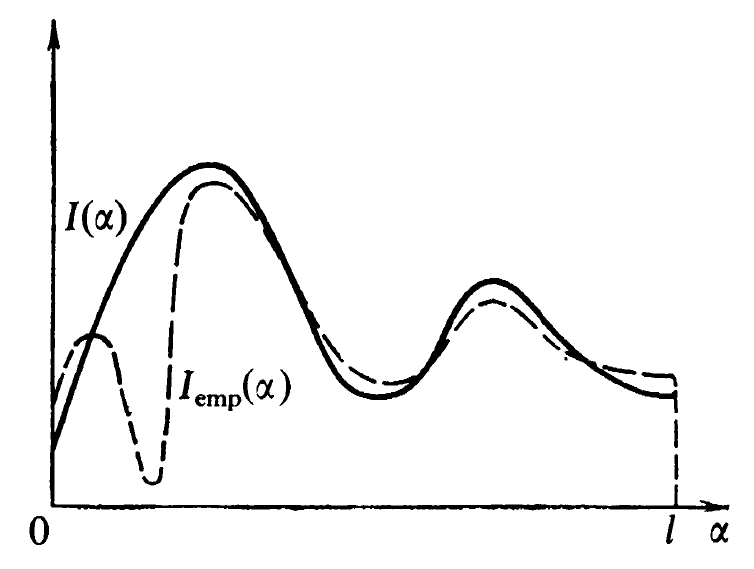
\includegraphics[width=.5\linewidth]{Img/chapter1/frequency.png}
\caption{机器学习理论一致收敛问题示意图}
\label{fig:frequency}
\end{figure}

\subsection{不可分情形下绝对偏差一致收敛的界}
\label{sec:special-case}

首先考虑不可分情形下“频率-概率”一致收敛的条件。考虑诸决策规则的类是由$N$个有限规则\footnote{这里的规则数目$N$是一个非常大的数 \citep{Lerner1980}。}组成的函数类$F(x;\alpha)$:
\begin{align}
F\left(x, \alpha_{1}\right), \ldots, F\left(x, \alpha_{N}\right).
\end{align}
对应每个决策规则$F(x,\alpha_i)$的随机事件$A_i$由数据对$x, y$组成, 且满足$(y - F(x,\alpha_i))^{2} = 1$。这就定义$N$个有限数量事件$A_1,\ldots,A_N$.

对于每个固定事件, 依照概率论易知大数定律自然是有效的, 即随着试验次数的无限增加, 此固定事件下的频率收敛至其概率。此大数定律的一个特例就是下列Hoffding不等式:
\begin{align}\label{ch6.15}
P\left\{\left|P\left(\alpha_{i}\right)-v\left(\alpha_{i}\right)\right|>\varkappa\right\}<2 \exp \left\{-2 \varkappa^{2} l\right\}.
\end{align}
然而, 要探究的核心在于要求一致收敛, 也就是说要求确保下列诸不等式同时满足的概率
\begin{align}
\left|P\left(\alpha_{i}\right)-v\left(\alpha_{i}\right)\right| \leq \varkappa, \quad i=1,2, \ldots, N.
\end{align}
如果对于表达式(\ref{ch6.15})中出现的每个不等式能够断言其可以独立分开评估的话, 那么一致收敛要求下的概率可以很容易地界定, 即可得
\begin{align}
P\left\{\sup _{i}\left|P\left(\alpha_{i}\right)-v\left(\alpha_{i}\right)\right|>\varkappa\right\} \leq \sum_{i=1}^{N} P\left\{\left|P\left(\alpha_{i}\right)-v\left(\alpha_{i}\right)\right|>\varkappa\right\}.
\end{align}
将不等式(\ref{ch6.15})带入,得到
\begin{align}\label{ch6.16}
P\left\{\sup _{i}\left|P\left(\alpha_{i}\right)-v\left(\alpha_{i}\right)\right|> \varkappa\right\}<2 N \exp \left\{-2 \varkappa^{2} l\right\}.
\end{align}
这个不等式就意味着, 对于有限数量的随机事件, 其“频率-概率”一致收敛始终有效, 也就是说其极限为
\begin{align}
\lim _{l \rightarrow \infty} P\left\{\sup _{i}\left|P\left(\alpha_{i}\right)-v\left(\alpha_{i}\right)\right|>\varkappa\right\}=0.
\end{align}

现在要求在特定事件的具体实现中,其对应的概率
\begin{align}
\left\{\sup _{i}\left|P\left(\alpha_{i}\right)-v\left(\alpha_{i}\right)\right|>\varkappa\right\}
\end{align}
不要超过$\eta$, 即要求下列表达式
\begin{align}\label{ch6.17}
P\left\{\sup _{i}\left|P\left(\alpha_{i}\right)-v\left(\alpha_{i}\right)\right|>\varkappa\right\}<\eta
\end{align}
需要成立。从不等表达式(\ref{ch6.16})中可以得到不等式(\ref{ch6.17})成立的条件是$N, l, \varkappa$ 和 $\eta$ 这些量化指标要满足下列关系式
\begin{align}\label{ch6.18}
2 N \exp \left\{-2 \varkappa^{2} l\right\}=\eta.
\end{align}
如果在表达式(\ref{ch6.18})中求解$\varkappa$, 那么对于给定的 $N, l$和$\eta$, 就得到在给定条件下的诸事件的类中, 诸频率与其概率的最大偏差的估计量就是
\begin{align}\label{ch6.19}
\varkappa=\sqrt{\frac{\ln N-\ln (\eta / 2)}{2 l}}.
\end{align}
然而, 如果在表达式(\ref{ch6.18})中解出$l$, 那么可以断言(assert), 至少以概率 (with probability) $1-\eta$ 在这个函数类上诸频率和诸概率的最大偏差不会超过$\varkappa$的样本的大小是:
\begin{align}\label{ch6.20}
l=\frac{\ln N-\ln (\eta / 2)}{2 \varkappa^{2}}.
\end{align}

因此证明下面的定理:
\begin{theorem}\label{theorem6.1}
\citep{vapnik1998}
设诸决策函数的集合包含$N$个元素, 对于决策函数$F(x,\alpha_i)$, 令在样本容量为$l$时分类错误的频率为$v(\alpha_i)$。那么, 以概率(with probability)$1-\eta$有可能断言(may assert)下列不等关系表达式,
\begin{align}
v\left(\alpha_{i}\right)-\sqrt{\frac{\ln N-\ln (\eta / 2)}{2 l}} \leq P\left(\alpha_{i}\right) \leq v\left(\alpha_{i}\right)+\sqrt{\frac{\ln N-\ln (\eta / 2)}{2 l}}
\end{align}
对于所有决策函数都同时成立。
\end{theorem}

\begin{remark}
因为以上不等式是对所有$N$个决策规则都成立, 因此定理 \ref{theorem6.1} 对于某个具体决策规则$F(x,\alpha_{\text{emp}})$——此规则在$N$个规则中能够最小化经验风险泛函——的品质确定其置信区间。这个置信区间就是
\begin{align}
v\left(\alpha_{\text {emp }}\right)-\sqrt{\frac{\ln N-\ln (\eta / 2)}{2 l}} \leq P\left(\alpha_{\text {emp }}\right) \leq v\left(\alpha_{\text {emp }}\right)+\sqrt{\frac{\ln N-\ln (\eta / 2)}{2 l}}.
\end{align}
\end{remark}

因为更关注决策规则的品质的上界, 即对于所有的决策规则, 以概率(with probability) $1-\eta$
\begin{align}
P\left(\alpha_{i}\right) \leq v\left(\alpha_{i}\right)+\sqrt{\frac{\ln N-\ln (\eta / 2)}{2 l}}
\end{align}
使得上面的不等式同时有效。

因此, 在决策规则有限情形下,一致收敛的要求不仅仅与最小化经验泛函$v(\alpha_{i})$有关, 还与决策规则的品质——即置信区间$\sqrt{\frac{\ln N-\ln (\eta / 2)}{2 l}}$——有关.

\subsection{可分情形下绝对偏差一致收敛的界}
\label{sec:kefen}
以上给出的是在一般决策规则有限的情形下考察的一致收敛问题。基于定理\ref{theorem6.1}计算得到的置信区间可能过于宽泛——因为在不可分情形下并不要求有限$N$个决策一定就包含那真实函数本身。

现在考虑可分情形下学习问题的一致收敛条件。因为在所有的决策函数$F(x,\alpha_i)(i=1,\ldots,N)$中确实存在着一个函数, 其能够完美地解决分类问题, 那么这就是一个明晰的先验知识, 即对于任意的样本其最小化经验风险泛函的值一定是0。然而, 这个最小值是可以通过好几个函数求得的。所以需要估计对于任意函数——这些函数都能够使得经验风险的最小值为0——其估计品质不超过给定的$\varkappa$的概率是多少。

引进函数
\begin{align}
\bar{\theta}(z)=\left\{\begin{array}{ll}
1 & \text { for } z=0 ,\\
0 & \text { for } z>0.
\end{array}\right.
\end{align}
那么, 在诸事件的集合上——在此集合上错误分类的频率为零——诸频率一致收敛至其概率的速度的估计, 就是针对下列事件的概率的估计
\begin{align}
\left\{\sup _{i}\left|P\left(\alpha_{i}\right)-v\left(\alpha_{i}\right)\right| \bar{\theta}\left(v\left(\alpha_{i}\right)\right)>\varkappa\right\}
\end{align}
(而并不是如定理\ref{theorem6.1}所述的针对事件$\left\{\sup _{i}\left|P\left(\alpha_{i}\right)-v\left(\alpha_{i}\right)\right| > \varkappa\right\}$的估计)。

因为对于那些使得经验风险取值为零的决策函数的数量不会超过$N$($N$是决策函数集合中函数的总数量), 所以下列不等式
\begin{align}\label{ch6.21}
P\left\{\sup _{i}\left|P\left(\alpha_{i}\right)-v\left(\alpha_{i}\right)\right| \bar{\theta}\left(v\left(\alpha_{i}\right)\right)>\varkappa\right\} \leq N P_{\varkappa}
\end{align}
总是成立的。其中, 这里$P_{\varkappa}$表征的是在所有样本中错误分类的误差超过$\varkappa$的概率。很自然地, 这一概率的界就由下列表达式给出
\begin{align}\label{ch6.22}
P_{\varkappa} \leq(1-\varkappa)^{l}.
\end{align}
将针对$P_{\varkappa}$的界带入表达式(\ref{ch6.21}), 得到
\begin{align}\label{ch6.23}
P\left\{\sup _{i}\left|P\left(\alpha_{i}\right)-v\left(\alpha_{i}\right)\right| \bar{\theta}\left(v\left(\alpha_{i}\right)\right)>\varkappa\right\} \leq N(1-\varkappa)^{l}.
\end{align}
为使得下列概率
\begin{align}
P\left\{\sup _{i}\left|P\left(\alpha_{i}\right)-v\left(\alpha_{i}\right)\right| \bar{\theta}\left(v\left(\alpha_{i}\right)\right)>\varkappa\right\}
\end{align}
不超过给定值$\eta$, 其充分条件便是下列表达式成立
\begin{align}\label{ch6.24}
N(1-\varkappa)^{l}=\eta.
\end{align}
从中求解$l$, 可得
\begin{align}\label{ch6.25}
l=\frac{\ln N-\ln \eta}{-\ln (1-\varkappa)}.
\end{align}
因为当$\varkappa$取较小值时, 下列近似表达式
\begin{align}
-\ln (1-\varkappa) \approx \varkappa
\end{align}
成立, 因此表达式(\ref{ch6.25})可以表示为下列形式
\begin{align}
l=\frac{\ln N-\ln \eta}{\varkappa}.
\end{align}
与表达式(\ref{ch6.20})不同的是, 这里得到的分母为$\varkappa$而不是先前得到的$2\varkappa^2$。这就是说, 在确定问题陈述中所需的样本量要比通常一般情况下的样本量少得多。在表达式(\ref{ch6.24})中求解$\varkappa$, 可以得到
\begin{align}
\varkappa=\frac{\ln N-\ln \eta}{l}.
\end{align}
这样便可以得到下列定理:

\begin{theorem}\label{theorem6.2}
\citep{vapnik1998}
如果在$N$个决策规则函数集合中可以选择出某一个规则,其能够使得样本分类不出错, 那么可以以概率(with probability)$1-\eta$断言(assert), 使用所选中的这一规则得到的错误分类概率的界为
\begin{align}
0 \leq P \leq \varkappa,
\end{align}
其中
\begin{align}
\varkappa=\frac{\ln N-\ln \eta}{l}.
\end{align}
\end{theorem}

从这里也可以看到, 即便是对于确定陈述问题, 最小化经验风险泛函的方法也不能够保证“频率-概率”一致收敛, “频率-概率”一致收敛仍然还要求控制决策规则的品质$\varkappa=\frac{\ln N-\ln \eta}{l}$。


\section{无限决策规则下学习问题一致收敛条件}
到目前为止, 已经在非常粗糙的层面通过使用“容量”来刻画诸决策规则的集合来得到“频率-概率”一致收敛速度的界(大概把“容量”等同于在此集合中诸元素的个数)。

在本节开始要引入一个更为精确的容量指标刻画量——样本大小$l$上诸事件的系统的熵。使用这一刻画指标可以全面而彻底详尽地阐发并建构随机事件“频率-概率”偏差一致收敛速度的充分必要条件, 即建构有关下列等式
\begin{align}
\lim _{l \rightarrow \infty} P\left\{\sup _{\alpha}|P(\alpha)-v(\alpha)|>\varkappa\right\}=0
\end{align}
对于任意$\varkappa$都成立的充分必要条件。

首先令诸决策规则$F(x,\alpha)$的集合$S$已被定义并且给定样本$x_1,\ldots,x_l$。这些样本一般说来当然可以按照$2^{l}$种方式划分为两类。然而, 只有可以使用诸规则$F(x,\alpha)$完成的那些划分才是感兴趣的。(也就是说, 感兴趣的是使用规则$F(x,\alpha^{*})$, 样本集合$x_1,\ldots,x_{l}$能够被划分为这样两个子集: 其一满足 $F(x,\alpha^{*})=1$, 另一集合满足$F(x,\alpha^{*})=0$。) 不同划分方法的数量依赖于诸决策规则$F(x,\alpha)$的类本身, 同时也依赖于样本。“不同划分方法的数量”这一指标记为
\begin{align}
\Delta^{S}\left(x_{1}, \ldots, x_{l}\right).
\end{align}

现在来考虑由诸决策规则$F(x,\alpha)$所构成的诸随机事件的系统
\begin{align}
S(\alpha)=\left\{x, y:(y-F(x, \alpha))^{2}=1\right\}.
\end{align}
对于给定随机独立样本
\begin{align}\label{ch6.36}
x_{1}, y_{1} ; \ldots ; x_{l}, y_{l}
\end{align}
随机事件系统$S(\alpha)$在样本(\ref{ch6.36})上便对应地可以诱导出 $\Delta\left(S(\alpha);x_{1}, w_{1};\ldots; x_{l},w_{l}\right)$种不同的子样本。显然, 这些子样本的数量就等于$\Delta^{S}(x_1,\ldots,x_{l})$。因为 $x_1,\ldots,x_l$是随机独立样本, 所以不同子划分的数量$\Delta^{S}(x_1,\ldots,x_{l})$也是随机变量。

现在给出一些与进一步阐述相关的定义。

\begin{definition}\citep{vapnik1998}
下列量化指标
\begin{align}
H^{S}(l)=M \ln \Delta^{S}\left(x_{1}, \ldots, x_{l}\right)
\end{align}
被称作是在样本量为$l$的随机样本上, 诸随机事件$S(\alpha)$的系统的\textsf{熵}。
\end{definition}

这样一来, 原来在诸事件的集合上频率$v(\alpha)$与其对应的概率$P(\alpha)$一致收敛的充分必要条件要求随着样本的增加, 单个元素引起的熵的占比逼近零。换言之, 随着样本量$l$增加, 下列序列
\begin{align}
\frac{H^{S}(1)}{1}, \frac{H^{S}(2)}{2}, \ldots, \frac{H^{S}(l)}{l}
\end{align}
逼近零。亦即要求下列条件
\begin{align}\label{ch6.37}
\lim _{l \rightarrow \infty} \frac{H^{S}(l)}{l}=0
\end{align}
要成立。

以上关于“频率-概率”一致收敛的充分必要条件时使用了一些提炼出来的概念。所谓“提炼”的意思就是说在提出的概念中多少是混合着一个没有彻底阐明的概念。此处提炼出来的概念正是这里阐述的“熵”的概念。在样本大小为$l$的样本上诸事件$S(\alpha)$的系统的熵, 是通过密度函数$P(x)$而建构起来的\citep{Kullback1968}。而对于模式识别问题这一密度函数$P(x)$是未知的。因此, 当利用这里提出的“熵”的概念时就无法绕过这个未被彻底澄清的概念。

为了获得具有建设性的充分条件, 就需要对此处熵的概念做微调。VC理论要求微调后的充分条件首先不依赖分布函数$P(x)$的属性, 其次还能够继续保持一致收敛速度的界。这样的充分条件可以用诸随机事件$S(\alpha)$的系统的一个容量测度来表征, 这一指标就是从熵$H^{S}(l)$中抽掉其与测度$P(x)$有关的属性而获得的。

现在来定义“容量测度”。

\begin{definition}\citep{vapnik1998}
下列函数是由诸决策函数$F(x,\alpha)$形成的系统的增长函数
\begin{align}
m^{S}(l)=\max _{x_{1}, \ldots, x_{l}} \Delta^{S}\left(x_{1}, \ldots, x_{l}\right).
\end{align}
\end{definition}

以如此这般的方式建构的增长函数是不再依赖测度$P(x)$属性, 并且同时下列不等式
\begin{align}\label{ch6.38}
\ln m^{S}(l) \geq H^{S}(l)
\end{align}
是总是成立的。现在如果下列表达式
\begin{align}
\frac{\ln m^{S}(l)}{l}
\end{align}
随着样本量$l$的增加而逼近零, 那么在表达式(\ref{ch6.38})的视野下, 比率$H^{S}(l)/l$逼近零那就更不用说。因此下列条件
\begin{align}
\lim _{l \rightarrow \infty} \frac{\ln m^{S}(l)}{l}=0
\end{align}
就是“频率-概率”一致收敛的充分条件\citep{vapnik1998,Alexey2015,Novoseltsev2015}。

\begin{theorem}\label{theorem6.6}
\citep{vapnik1998}
增长函数要么等于$2^{l}$, 要么当$l>h$时, 增长函数被下列函数主宰
\begin{align}
m^{S}(l)<1.5 \frac{l^{h}}{h !},
\end{align}
其中, 这里的$h+1$是使得条件$m^{S}(l)=2^{l}$不成立时的最少的样本量。换言之,
\begin{align}
m^{S}(l)\left\{\begin{array}{l}
\text{要么} \equiv 2^{l} ,\\
\text{要么} <1.5 \frac{l^{h}}{h !} \quad(l>h).
\end{array}\right.
\end{align}
\end{theorem}

也就是说, 为界住一个增长函数, 所需的正就是要表明,
\begin{enumerate}
\item[(1)] 要么, 对于任意的$l$个样本$x_1,\ldots,x_l$, 使用这些诸决策规则$F(x, \alpha)$其能够将之用任意的$2^l$种方式其中之一将这些样本划分成两类;
\item[(2)] 要么, 就一定会存在这样一个数——这个数记为$h$——使得对于$h$个数据点是可以以所有可能的划分方式分开的, 但是当有$h+1$个数据点时, 就无法分开。
\end{enumerate}

\begin{definition}\citep{vapnik1998}
诸示性函数的类本身拥有容量$h$, 就是说, 如果下列不等式
\begin{align}\label{ch6.39}
m^{S}(l)<1.5 \frac{l^{h}}{h !} \quad(l>h)
\end{align}
是成立的。 如果是下列等式
\begin{align}
m^{S}(l) \equiv 2^{l}
\end{align}
成立, 那么诸示性函数$F(x,\alpha)$的类本身的容量$h$是无限。
\end{definition}

有容量的概念后, 很容易确认如果诸示性函数的类的容量是有限的, 那么“频率-概率”一致收敛就总是成立的。 确实在这种情形下, 下列关系表达式
\begin{align}
0 \leq \lim _{l \rightarrow \infty} \frac{\ln m^{S}(l)}{l} \leq \lim _{l \rightarrow \infty} \frac{h \ln l-\sum_{i=1}^{h} \ln i}{l}=0
\end{align}
的确是成立的并且其充分条件也是满足的\citep{vapnik1998}。

\subsection{“频率-概率”一致收敛速度的界}
\label{sec:rate-of-convergence}
根据\citet{Vapnik2006}, 前面的章节中完成对容量概念的引进, 也给出基于这一概念对“频率-概率”一致收敛的证明, 在本节基于诸决策规则的集合的容量概念, 给出“频率-概率”一致收敛速度的界。 

根据VC理论, 下列表达式
\begin{align}\label{ch6.41}
P\left\{\sup _{\alpha}|P(\alpha)-v(\alpha)|>\varkappa\right\}<6 m^{S}(2 l) \exp \left\{-\frac{\varkappa^{2} l}{4}\right\}
\end{align}
是成立的。 界(\ref{ch6.41})与上文中介绍的各类界有着形式上的统一: 就其形式而言, 正就是通过乘以——$6m^{S}(2l)$——这一刻画诸随机事件的类的容量, 从而使得“频率-概率”偏差界不超过$\varkappa$。

如果诸决策函数的类的容量是无限($m^{S}(l) \equiv 2l$), 那么得到的界(\ref{ch6.41})就是平凡的, 因为对于所有的$\varkappa$不等式的右边都大于1。 要求界(\ref{ch6.41})有具体的意义, 只有当诸决策规则的类的容量是有限的情况下才成立, 即要求
\begin{align}
m^{S}(l)<1.5 \frac{l^{h}}{h !}.
\end{align}
在这种情况下, 其应有的形式是
\begin{align}\label{ch6.42}
P\left\{\sup _{\alpha}|P(\alpha)-v(\alpha)|>\varkappa\right\}<9 \frac{(2 l)^{h}}{h !} \exp \left\{-\frac{\varkappa^{2} l}{4}\right\}.
\end{align}
随着$l$的增加, 不等式(\ref{ch6.42})的右边趋近于0并且对于容量$h$较小值情形下(此时其起作用的正是不等式右侧项的指数项)其以更快的速度逼近。 要求概率
\begin{align}
P\left\{\sup _{\alpha}|P(\alpha)-v(\alpha)|>\varkappa\right\}
\end{align}
不能超过$\eta$。 那么就是要求下列等式要成立, 即
\begin{align}\label{ch6.43}
9 \frac{(2 l)^{h}}{h !} \exp \left\{-\frac{\varkappa^{2} l}{4}\right\}=\eta.
\end{align}
由等式(\ref{ch6.43})可以解出$\varkappa$(使用斯特林公式(Stirling's formula)):
\begin{align}\label{ch6.44}
\varkappa=2 \sqrt{\frac{h\left(\ln \frac{2 l}{h}+1\right)-\ln \frac{\eta}{9}}{l}}.
\end{align}
那么由表达式(\ref{ch6.42})-(\ref{ch6.44})可以得到下列的定理:

\begin{theorem}\label{Theorem6.7}\citep{vapnik1998}
令$F(x, \alpha)$是被容量$h$界住的诸决策规则的这些类, $v(\alpha)$是利用此规则$F(x,\alpha)$从这些样本计算的误差的频率。 那么有可能断言, 对于所有的决策规则$F(x,\alpha)$, 当满足$l>h$的情形时, 以概率 (with probability) $1-\eta$错误分类的概率以下列形式被界住:
\begin{equation*}
\begin{aligned}
v(\alpha)&-2 \sqrt{\frac{h\left(\ln \frac{2 l}{h}+1\right)-\ln \frac{\eta}{9}}{l}} \\
&<P(\alpha)<v(\alpha)+2 \sqrt{\frac{h\left(\ln \frac{2 l}{h}+1\right)-\ln \frac{\eta}{9}}{l}}.
\end{aligned}
\end{equation*}
\end{theorem}

基于表达式(\ref{ch6.41}), 还可以得到“频率-概率”相对一致收敛界
\begin{align}
P\left\{\sup _{\alpha} \frac{P(\alpha)-v(\alpha)}{\sqrt{P(\alpha)}}>\varkappa\right\}<8 m^{S}(2 l) e^{-\varkappa^{2} l / 4}
\end{align}
也是成立的。 这一界对于有限容量的诸决策规则的类是非平凡的, 即下列不等关系成立
\begin{align}\label{ch6.45}
P\left\{\sup _{\alpha} \frac{P(\alpha)-v(\alpha)}{\sqrt{P(\alpha)}}>\varkappa\right\}<12 \frac{(2 l)^{h}}{h !} e^{-\varkappa^{2} l / 4}.
\end{align}

现在需要确认这一界的右边部分等于$\eta$:
\begin{align}
12 \frac{(2 l)^{h}}{h !} e^{-\varkappa^{2} l / 4}=\eta.
\end{align}

显然如果满足下列关系:
\begin{align}\label{ch6.46}
\varkappa=2 \sqrt{\frac{\ln \frac{(2 l)^{h}}{h !}-\ln \frac{\eta}{12}}{l}} \approx 2 \sqrt{\frac{h\left(\ln \frac{2 l}{h}+1\right)-\ln \frac{\eta}{12}}{l}}.
\end{align}
就是自然成立的。 另一方面, 不等关系(\ref{ch6.45})还可以做如下的称述, 即以概率 (with probability) $\eta$, 对于所有的$\alpha$下列不等关系
\begin{align}\label{ch6.47}
P(\alpha) \leq \frac{\varkappa^{2}}{2}\left(1+\sqrt{1+\frac{4 v(\alpha)}{\varkappa^{2}}}\right)+v(\alpha)
\end{align}
同时成立。 根据表达式(\ref{ch6.46})和表达式(\ref{ch6.47})之间的关系可推导出下列定理。

\begin{theorem}\label{Theorem6.8}\citep{vapnik1998}
令$F(x, \alpha)$是被容量$h$界住的诸决策规则的一个类, 对于每个规则$F(x,\alpha)$, 设其就在这样本中计算得到的误差的频率为$v(\alpha)$。 那么以概率 (with probability) $1-\eta$可以断言 (assert), 下列界
\begin{align}\label{ch6.48}
P(\alpha) \leq 2 \frac{h\left(\ln \frac{2 l}{h}+1\right)-\ln \frac{\eta}{12}}{l}\left(1+\sqrt{1+\frac{v(\alpha) l}{h\left(\ln \frac{2 l}{h}+1\right)-\ln \frac{\eta}{12}}}\right)+v\left(\alpha_{\text {emp }}\right)
\end{align}
当$l>h$时对于在这类中的所有的决策规则都同时成立。
\end{theorem}

这样一来, 使用精确定义的诸决策规则的类的容量概念, 不仅仅得到“频率-概率”一致收敛的充要条件: 诸决策规则函数的类的VC维有限; 而且还得到“频率-概率”一致收敛速度的界: 也要求诸决策规则函数的类的VC维有限。

\section{本章小结}
本章将学习问题的理论归约为最小化经验风险泛函, 分析机器学习算法一致收敛的充分必要条件, 并指出只有保证“频率-概率”一致收敛才能确保最小化经验风险泛函取得最佳估计。 主要结论总结如下:
\begin{enumerate}
\item 从有限决策规则出发, 分别阐述不可分情形和可分情形下机器学习算法一致收敛的条件。分析结果指明, 必须控制两个因子(经验风险最小化和机器的容量)才能使得经验风险泛函取得最佳估计;
\item 将有限决策规则情形推广至无限决策规则, 并将机器的容量精确定义为机器的VC维, 得到学习问题一致收敛的充分必要条件是VC维有限;
\item 在VC维理论基础上得到学习问题一致收敛速度的界。这一理论结果表明, 无论是学习问题一致收敛的充分必要条件还是学习问题一致收敛速度的界, 都由机器的VC维唯一确定。
\end{enumerate}